

%===================================================================================================
%	DOCUMENT DEFINITION
%===================================================================================================

%we use article class because we want to fully customize the page and dont use a cv template
\documentclass[10pt,a4paper]{article}	

%---------------------------------------------------------------------------------------------------
%	ENCODING
%---------------------------------------------------------------------------------------------------

%we use utf8 since we want to build from any machine
\usepackage[utf8]{inputenc}		

%---------------------------------------------------------------------------------------------------
%	LOGIC
%---------------------------------------------------------------------------------------------------

% provides \isempty test
\usepackage{xifthen}

%---------------------------------------------------------------------------------------------------
%	FONT
%---------------------------------------------------------------------------------------------------

% some tex-live fonts - choose your own

%\usepackage[defaultsans]{droidsans}
%\usepackage[default]{comfortaa}
%\usepackage{cmbright}
%\usepackage[default]{raleway}
%\usepackage{fetamont}

\usepackage[default]{gillius}

%\usepackage[light,math]{iwona}
%\usepackage[thin]{roboto}
\usepackage{hyperref}

% set font default
\renewcommand*\familydefault{\sfdefault} 	
\usepackage[T1]{fontenc}

% more font size definitions
\usepackage{moresize}		

%---------------------------------------------------------------------------------------------------
%	PAGE LAYOUT  DEFINITIONS
%---------------------------------------------------------------------------------------------------

%debug page outer frames
%\usepackage{showframe}			

%define page styles using geometry
\usepackage[a4paper]{geometry}		

% for example, change the margins to 2 inches all round
\geometry{top=1.75cm, bottom=1.0cm, left=1.5cm, right=1.5cm} 	

%use customized header
\usepackage{fancyhdr}		
\pagestyle{fancy}

%less space between header and content
\setlength{\headheight}{-5pt}		

%customize entries left, center and right
\lhead{}
\chead{\small{
  Khalid Al-Khatib $\cdot$ 
  Assistant Professor in NLP $\cdot$ 
  Groningen, Netherlands $\cdot$ 
  \textcolor{sectcol}{\textbf{\href
  {mailto:khalid.alkhatib@rug.nl}
  {khalid.alkhatib@rug.nl}}}
 $\cdot$ +31 6 31984076
}}
\rhead{}

%indentation is zero
\setlength{\parindent}{0mm}

%---------------------------------------------------------------------------------------------------
%	TABLE /ARRAY DEFINITIONS
%--------------------------------------------------------------------------------------------------- 

%for layouting tables
\usepackage{multicol}			
\usepackage{multirow}

%extended aligning of tabular cells
\usepackage{array}
\newcolumntype{x}[1]{>{\raggedleft\hspace{0pt}}p{#1}}

%---------------------------------------------------------------------------------------------------
%	GRAPHICS DEFINITIONS
%--------------------------------------------------------------------------------------------------- 

%for header image
\usepackage{graphicx}

%for floating figures
\usepackage{wrapfig}
\usepackage{float}
%\floatstyle{boxed} 
%\restylefloat{figure}

%for drawing graphics		
\usepackage{tikz}				
\usetikzlibrary{shapes, backgrounds,mindmap, trees}

%---------------------------------------------------------------------------------------------------
%	Color DEFINITIONS
%--------------------------------------------------------------------------------------------------- 

\usepackage{color}

%accent color
\definecolor{sectcol}{RGB}{160,160,160}


%dark background color
\definecolor{bgcol}{RGB}{0,153,0}


%light background / accent color
\definecolor{softcol}{RGB}{120,140,60}



%===================================================================================================
%	DEFINITIONS
%===================================================================================================

%---------------------------------------------------------------------------------------------------
% 	HEADER
%---------------------------------------------------------------------------------------------------

% remove top header line
\renewcommand{\headrulewidth}{0pt} 

%remove botttom header line
\renewcommand{\footrulewidth}{0pt}	  	

%remove pagenum
\renewcommand{\thepage}{}	

%remove section num		
\renewcommand{\thesection}{}			

%---------------------------------------------------------------------------------------------------
% 	ARROW GRAPHICS in Tikz
%---------------------------------------------------------------------------------------------------

% a six pointed arrow poiting to the left
\newcommand{\tzlarrow}{(0,0) -- (0.2,0) -- (0.3,0.2) -- (0.2,0.4) -- (0,0.4) -- (0.1,0.2) -- cycle;}	

% include the left arrow into a tikz picture
% param1: fill color
%
\newcommand{\larrow}[1]{
  \begin{tikzpicture}[scale=0.58]
    \filldraw[fill=#1!100,draw=#1!100!black]  \tzlarrow
  \end{tikzpicture}
}

% a six pointed arrow poiting to the right
\newcommand{\tzrarrow}{ (0,0.2) -- (0.1,0) -- (0.3,0) -- (0.2,0.2) -- (0.3,0.4) -- (0.1,0.4) -- cycle;}

% include the right arrow into a tikz picture
% param1: fill color
%
\newcommand{\rarrow}{
  
\begin{tikzpicture}[scale=0.7]
    \filldraw[fill=sectcol!100,draw=sectcol!100!black] \tzrarrow
  \end{tikzpicture}
}
%---------------------------------------------------------------------------------------------------
%	custom sections
%---------------------------------------------------------------------------------------------------

% create a coloured box with arrow and title as cv section headline
% param 1: section title
%
\newcommand{\cvsection}[1]{
  \vspace{10pt}
  \colorbox{sectcol}{\mystrut \makebox[1\linewidth][l]{
    \larrow{bgcol} \hspace{-8pt} \larrow{bgcol} \hspace{-8pt} 
    \larrow{bgcol}\textcolor{white}{\textbf{#1}}\hspace{4pt}
  }}\\
}

%create a coloured arrow with title as cv meta section section
% param 1: meta section title
%
\newcommand{\metasection}[2]{
  \begin{tabular*}{1\textwidth}{p{2.4cm} p{14cm}}
    \larrow{bgcol} \normalsize{\textcolor{bgcol}{#1}}&#2\\[10pt]
  \end{tabular*}
}

%---------------------------------------------------------------------------------------------------
%	 CV EVENT
%---------------------------------------------------------------------------------------------------

% creates a stretched box as cv entry headline followed by two paragraphs
% param 1:	event time i.e. 2014 or 2011-2014 etc.
% param 2:	event name (what did you do?)
% param 3:	institution (where did you work / study)
%
\newcommand{\cvevent}[3]{
  \begin{tabular*}{1\textwidth}{p{2.4cm} p{6.5cm} x {8.0cm}}
    \textcolor{bgcol}{#1} & \textbf{#2} & \vspace{2.5pt}\textcolor{bgcol}{#3}
  \end{tabular*}
  \vspace{-10pt}
  \textcolor{softcol}{\hrule}
  \vspace{10pt}
}

% creates a stretched box as cv entry detail 
% param 1:	information describing the event
%
\newcommand{\cvdetail}[1]{
  \begin{tabular*}{1\textwidth}{p{2.5cm} p{14.5cm}}
    & \larrow{bgcol}  #1\\ [3pt]
  \end{tabular*}
}

%---------------------------------------------------------------------------------------------------
% CUSTOM STRUT FOR EMPTY BOXES
%---------------------------------------------------------------------------------------------------
\newcommand{\mystrut}{\rule[-.3\baselineskip]{0pt}{\baselineskip}}

%===================================================================================================
%	DOCUMENT CONTENT
%===================================================================================================
\title{resume}
\begin{document}

% use our custom fancy header definitions
\pagestyle{fancy}	

%---------------------------------------------------------------------------------------------------
%	TITLE HEADLINE
%---------------------------------------------------------------------------------------------------

\vspace{-20pt}

% use this for single words, e.g. CV or RESUME etc.
\hspace{-0.25\linewidth}\colorbox{bgcol}{
  \makebox[1.5\linewidth][c]{
    \HUGE{\textcolor{white}{\textsc{Khalid Al-Khatib}}} 
    \textcolor{sectcol}{\rule[-1mm]{1mm}{0.9cm}} 
    \HUGE{\textcolor{white}{\textsc{}}}
  }
}

%---------------------------------------------------------------------------------------------------
%	HEADER IMAGE
%---------------------------------------------------------------------------------------------------

%\begin{figure}[H]
%\begin{flushright}
 % 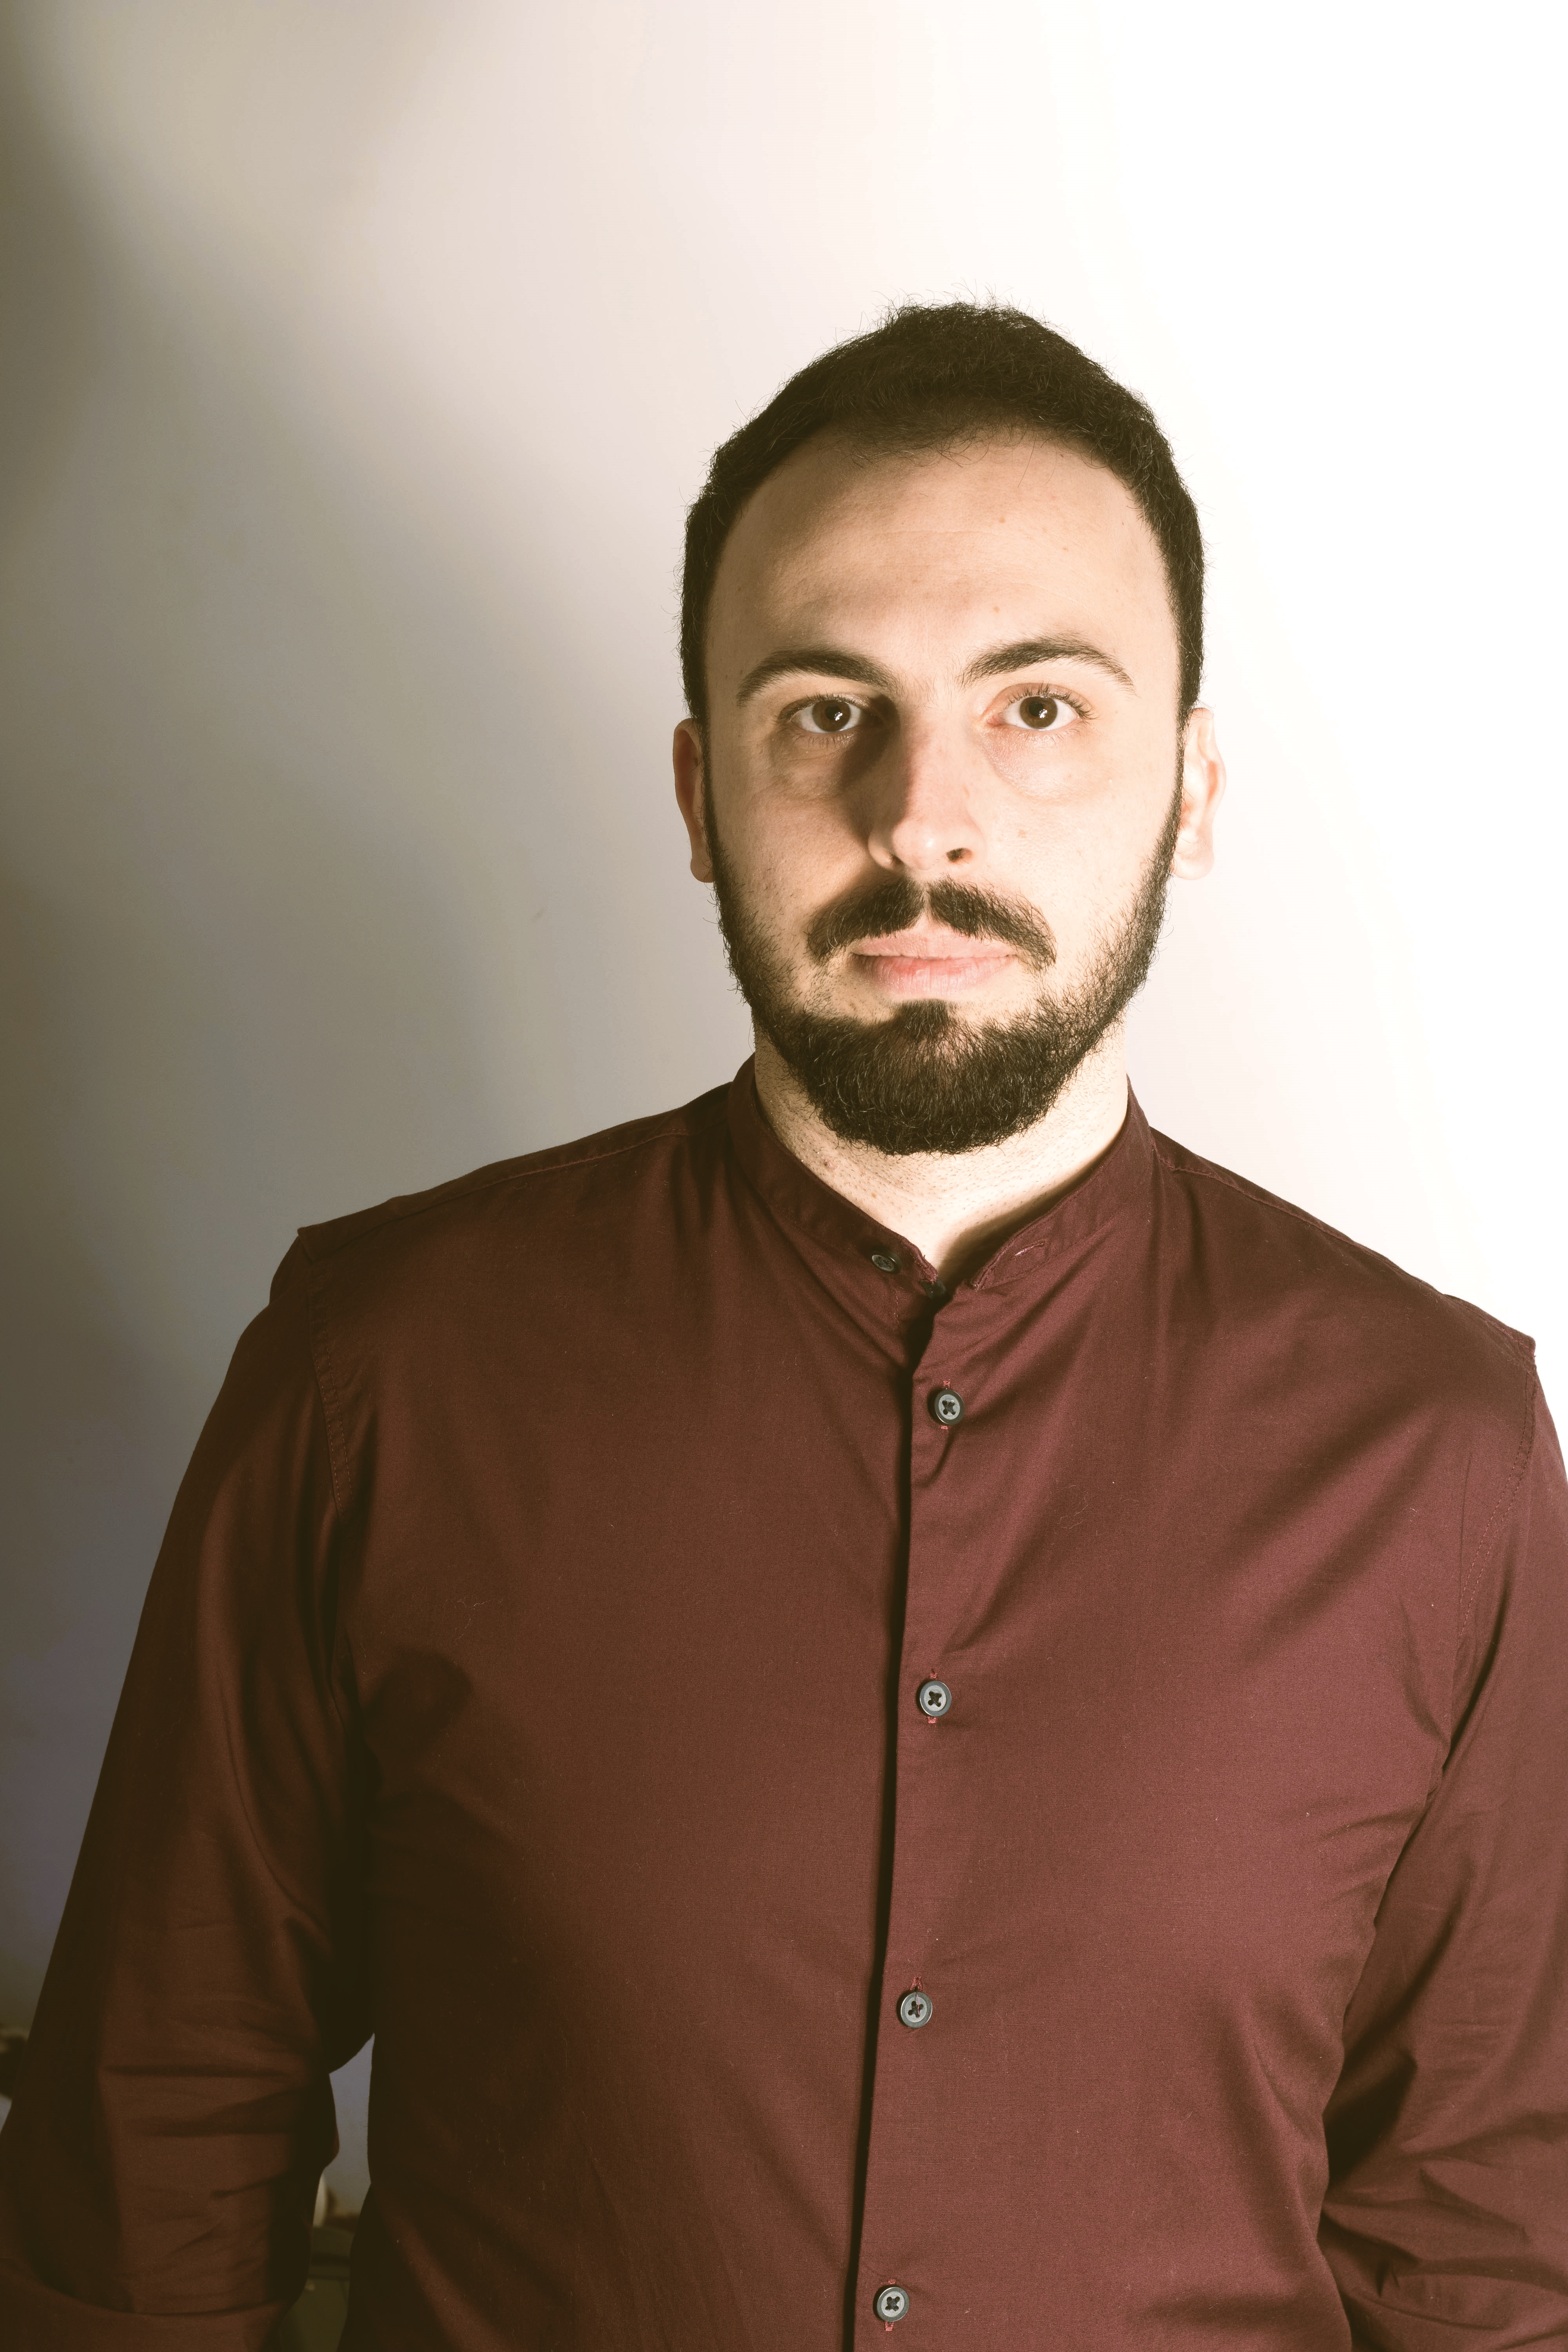
\includegraphics[width=0.2\linewidth]{khalid.jpg}
%\end{flushright}
%\end{figure}

%---------------------------------------------------------------------------------------------------
%	META SECTION
%---------------------------------------------------------------------------------------------------

%\vspace{-115pt}

%\metasection{Status:}{Developer at The Company, M.Sc. in Computer Science}
%\metasection{Skills:}{Java, C\#/.Net, C++, Python, JavaScript, Ruby, Bash, SQL} 
%\metasection{Interests:}{Data Warehouses, Data Lakes, Data Analysis, Data Quality}
%\metasection{Activities:}{Hockey, Football, Tennis, Basketball, Reading, Music}

%---------------------------------------------------------------------------------------------------
%	SUMMARAY (optional)
%---------------------------------------------------------------------------------------------------

% Short research focus and persistent academic identifiers
\metasection{Research:}{Computational argumentation, human--AI deliberation, argument quality assessment, argumentation knowledge graphs, and Arabic NLP.}
\metasection{Profiles:}{\href{https://orcid.org/0009-0006-7255-5349}{ORCID} $\cdot$ \href{https://research.rug.nl/en/persons/khalid-al-khatib/}{RUG Research Portal} $\cdot$ \href{https://dblp.org/pid/31/8936.html}{DBLP} $\cdot$ \href{https://github.com/Khalid-AlKhatib}{GitHub}}


%===================================================================================================
%	CV SECTIONS AND EVENTS (MAIN CONTENT)
%===================================================================================================

%---------------------------------------------------------------------------------------
%	EXPERIENCE
%----------------------------------------------------------------------------------------
\cvsection{Experience}


%\textcolor{softcol}{\hrule}

\cvevent
{01.2022-}
{Assistant Professor}
{University of Groningen}
\cvdetail{Research on computational argumentation, human--AI deliberation, argument quality, and Arabic NLP; lead researcher for the EU-funded AKASE project (2025--2026).}

\cvevent
{11.2020 - 12.2021}
{Postdoctoral Researcher}
{Leipzig University}
%\cvdetail{Advisor: Prof. Dr. Martin Potthast}

\cvevent
{01 - 10.2020}
{Postdoctoral Researcher}
{Martin-Luther-University, Bauhaus-Universität Weimar}
%\cvdetail{Advisor: Prof. Dr. Matthias Hagen, Prof. Dr. Benno Stein}

\cvevent
{2015 - 2019} % Date(s)
{Researcher} % Job title
{Bauhaus-Universität Weimar}
%\cvdetail{Advisor: Prof. Dr. Benno Stein}


\cvevent
{11.2018 - 04.2019} % Date(s)
{Research Intern} % Job title
{IBM Research, Ireland Research Lab} % Organization
%\cvdetail{Advisor: Dr. Yufang Hou}

\cvevent
{2011 - 2013} % Date(s)
{Researcher} % Job title
{Institute for NLP, University of Stuttgart}
%\cvdetail{Advisor: Prof. Dr. Hinrich Schutze, Prof. Dr. Cathleen Kantner.}

%---------------------------------------------------------------------------------------
%	EDUCATION SECTION
%--------------------------------------------------------------------------------------
\cvsection{Education}




\cvevent
{2014 - 2019} 
{PhD in Computer Science}
{Bauhaus-Universität Weimar} 
\cvdetail{{ \href{https://e-pub.uni-weimar.de/opus4/frontdoor/deliver/index/docId/4461/file/diss-alkhatib-frame.pdf} {Dissertation: ``Computational Analysis of Argumentation Strategies''}}
}
\cvdetail{Advisor: {\href{https://www.uni-weimar.de/en/media/institutes/digital-bauhaus-lab/people/prof-dr-benno-stein/} {Prof. Dr. Benno Stein}}. External examiner: {\href{https://www.ling.uni-potsdam.de/~stede/} {Prof. Dr. Manfred Stede}}
}



%------------------------------------------------

%------------------------------------------------

\cvevent
{2007 - 2010}
{MS. in Computer Science} % Degree
{Jordan University of Science \& Tech.}
%\cvdetail{GPA: 87.1\% (Very Good). Rank: top 5\%.}
%------------------------------------------------

%------------------------------------------------

\cvevent
{2008 - 2009} % Date(s)
{Visiting Graduate Student} % Degree
{Masaryk University} % Institution
%\cvdetail{Graduate level courses in Computer Science.} {}
%------------------------------------------------
%------------------------------------------------

%\cvevent
%{2003 - 2007} % Date(s)
%{BSc. in Computer Science} % Degree
%{Al Balqa Applied University} % Institution
%\cvdetail{GPA: 3.28/4.00 (Very Good). Rank: top 5\%.}{}

%------------------------------------------------

%%---------------------------------------------------------------------------------------
%	Honors \& Awards
%--------------------------------------------------------------------------------------
\cvsection{Research Projects}


\cvevent
{2020 - Present}
{Conversational News}
{Martin-Luther-University, Bauhaus-Universität Weimar} % 
\cvdetail{This project includes the development of a prototype that deploy text news articles to smart assistants. Writing augmented tools will be provided by semi-automatic ways to enhance the experience of delivering news in audio channels.}
\cvdetail{The project is funded by Google within the Digital News Innovation Fund.}

\cvevent
{2019 - Present}
{Argumentation Knowledge Graph}
{Bauhaus-Universität Weimar (Webis.de)} %
\cvdetail {The project aims for constructing an argumentation knowledge graph that is adequate for supporting several artificial intelligent down-stream applications such as text generation, decision making, and argument search.}
\cvdetail{The project is partially funded by IBM through the Ph.D. fellowship award.}

\cvevent
{2015 - 2018}
{Args.me Search Engine}
{Bauhaus-Universität Weimar (Webis.de)} %
\cvdetail {This project targets the development of the first argument search engine on the web. The project addresses several challenges of mining arguments and their relations from natural language text on the web. We develop algorithms that (1) robustly tackle various forms of web argumentation, (2) efficiently leverage the scale of the web, and (3) effectively complement argument mining with an argumentation analysis to assess important quality dimensions.}
\cvdetail{The project is funded by the German Research Foundation (DFG).}
\cvdetail{Advisor: Prof. Dr. Benno Stein. Prof. Dr. Matthias Hagen, Jun. Prof. Dr. Henning Wachsmuth}

\cvevent
{2015 - Present}
{Argumentation Strategies}% Job title
{Bauhaus-Universität Weimar (Webis.de)} %
\cvdetail {This research project is centered around the strategies that authors of monological argumentative texts, such as news editorials and scientific articles, employ to persuade their readers. It seeks to (1)~establish computational models of such argumentation strategies, (2)~analyze what strategies are common and effective within and across argumentative text genres, and (3)~synthesize texts with effective strategies for given sets of arguments.}
\cvdetail{The project is funded by the German Research Foundation (DFG).}
\cvdetail{Advisor: Prof.Dr. Benno Stein. Jun.-Prof. Dr. Henning Wachsmuth.}

\cvevent
{11.2018 - 04.2019} % Date(s)} 
{Counter-argument Generation} 
{IBM Research, Ireland Research Lab}
\cvdetail {This project concerns developing new technologies for tackling the following task:given a target argument, we aim to recommend its counterargument(s) from a set of mined arguments related to the same topic.}
\cvdetail{Advisor: Dr. Lea Deleris. Dr. Yufang Hou}

\cvevent
{2011-2013} 
{Sentiment Topic Analysis} 
{Institute for NLP, University of Stuttgart} 
\cvdetail {This project studies some areas in sentiment analysis that haven’t been studied extensively before like perspectives’ classification, bias detection, and the relation between social networks and their users with the public opinion of different sub-communities.}
\cvdetail{Advisor: Prof. Dr. Hinrich Schutze.}

\cvevent
{2011-2013} 
{eIdentity} 
{Institute for NLP, University of Stuttgart} 
\cvdetail {This project studies multiple collective identities in international debates about war and peace since the end of the Cold War. Many language technology tools
and methods are used to analyze multilingual text concepts in the social sciences.}
%My Role: I work on mining Wikipedia tables and extracting of temporal facts about politicians.\\
\cvdetail{Advisor: Prof. Dr. Cathleen Kantner.}

%---------------------------------------------------------------------------------------
%	Honors \& Awards
%--------------------------------------------------------------------------------------
\cvsection{Honors \& Awards}

\cvevent
{2025} 
{ \href{https://qatardebate.org/programs/academic-programs/qdfellowship/}
      {QatarDebate Fellowship}} % Award
{QatarDebate Center\\} % Event

\cvevent
{2025} 
{ \href{https://www.rug.nl/jantina-tammes-school/research/funding-grants-prizes/jts-early-career-researcher-prize?lang=en}
      {JTS Early Career Researcher Prize }} % Award
{Jantina Tammes School of Digital Society, Technology \\} % Event

%------------------------------------------------

\cvevent
{2017} 
{ \href{https://www.research.ibm.com/university/awards/fellowships.html}
      {IBM Ph.D. Fellowship Award}} % Award
{IBM} % Event

%------------------------------------------------

\cvevent
{2011 - 2012} % Date(s)
{SFB 732 Research Scholarship} % Award
{University of Stuttgart} % Event


%------------------------------------------------

\cvevent
{2008 - 2009} % Date(s)
{Erasmus Mundus Action2 Scholarship} % Award
{Masaryk University} % Event


%------------------------------------------------

\cvevent
{2009 - 2010} % Date(s)
{Graduate Scholarship} % Award
{Jordan University of Science and Technology} % Event



%---------------------------------------------------------------------------------------
%   Organisation
%--------------------------------------------------------------------------------------
\cvsection{Organisation}


\metasection{Workshop}{


\begin{itemize}

 \item Co-organizer of the Lorentz workshop: \href{https://www.lorentzcenter.nl/hybrid-argumentation-and-responsible-ai.html} {Hybrid Argumentation and Responsible AI
}.
 
\item Co-chair of the \href{http://www.vis4nlp.com/} {First Workshop on Visualization for Natural Language Processing (Vis4NLP)}.

 \item Co-organizer of the Dagstuhl seminar: \href{https://www.dagstuhl.de/en/program/calendar/semhp/?semnr=22432} {Towards a Unified Model of Scholarly Argumentation}.
 \item Co-chair of \href{https://2021.argmining.org} {the 8th Workshop on Argument Mining}.
 \item Co-chair of the \href{https://argkg21.argmining.org/} {first Workshop on Argumentation Knowledge Graphs}. 
\end{itemize}
  
}
\metasection{Tutorial}{Co-presenter of the \href{http://ratio.sc.cit-ec.uni-bielefeld.de/de/events/ki-tutorial-21-25-sep-2020/} {Argumentation Technology for AI' tutorial in the 43rd German Conference on Artificial Intelligence}, 2020
} 
\metasection{Shared Task}{Co-organiser of the \href{https://webis.de/events/sameside-19/}{Same-Side Stance} shared task on ArgMining workshop, 2019.




}


%---------------------------------------------------------------------------------------
%   Reviewing
%--------------

\cvsection{Reviewing}

\metasection{Conference:}{\textit{Reviewer}: ACL: 2016-2024, AAAI: 2019, NAACL: 2016, 2019. COLING: 2018, 2020. EMNLP: 2017, 2019, 2020. EACL: 2016. \newline \textit{Area Chair}: EMNLP:2025, 2025, ACL: 2023, 2025 COLING: 2022, 2024, 2025. EACL: 2023 
}
\metasection{Workshop:}{ArgMining Workshop: 2016-2024} 
\metasection{Journal:}{Language Resources and Evaluation: 2021, Artificial Intelligence: 2022,  Natural Language Engineering: 2022. Argument \& Computation: 2023, The Journal of Artificial Intelligence Research (JAIR): 2024.} 


\cvsection{Grants}

\begin{enumerate}
\item \href{https://openwebsearch.eu}{OpenWebSearch.EU} Project’s Third-Party; 97k, one year, 2024.
\item \href{https://enlight-eu.org}{ENLIGHT} ENLIGHT+ call; 1k, 2024.
%\item \href{https://openwebsearch.eu}{OpenWebSearch.EU} Project’s Third-Party; 97k, one year, 2024.


\item {}
\end{enumerate}
\cvsection{Invited Talks}

\begin{enumerate}
\item Invited research talk, \href{https://www.ai.uni-hannover.de/en/teaching/seminars/ai-nlp}{Graduate Seminar in Artificial Intelligence and Natural Language Processing}, Leibniz University Hannover, Germany, 12 December 2022.
\end{enumerate}

%---------------------------------------------------------------------------------------
%   Supervision
%--------------
\cvsection{Teaching and Supervision}

\cvevent
{2022-} % Date(s)
{Teaching} % Affiliation/role
{University of Groningen, Netherlands} % Organization/group
\begin{enumerate}
\item Introduction to Programming I (Bachelor)
\item Introduction to Programming II (Bachelor)
\item Project Text Analysis (Bachelor)
\item Web Programming (Bachelor)
\item Information Science BA Thesis\&Res.Se (Bachelor)
\item Language Technology Project (Master) 
\end{enumerate}
\cvevent
{2015 - 2016} % Date(s)
{Seminar Advising} % Affiliation/role
{Bauhaus-Universität Weimar} % Organization/group

\begin{enumerate}
\item {Advanced Topics in Information Retrieval and Natural Language Processing. (Winter 2015)}
\item {Advanced Topics in Information Retrieval and Natural Language Processing. (Summer 2015)}
\end{enumerate}


\cvevent
{2015-2022} % Date(s)
{Student Theses Supervision} % Affiliation/role
{Weimar, Leipzig, Groningen} % Organization/group


Master Theses:
\begin{enumerate}
\item Behrooz Nikandish, Identifying Effective Deliberation Strategies in Wikipedia Talk Pages
\item Vishal Khanna. Identifying Debating Strategies in Persuasive Discussions.
\item Christian Staudte. Generating Arguments Depending on Argumentation Schemes.
\item Dipendra Sharma Kafle. Style-based Analysis of Persuasive Strategies. 
\item Fan Fan: Mining High-ethos Evidence from Wikipedia.
\item Fatema Merchant: Neural Paraphrasing Methods for Augmented Writing Tools.
\item Anh Phuong Le, Harvesting the Web for Building Large-scale Argumentation Graphs.
\item Nikolay Kolyada, Author or Argumentation: Exploring the Effect of Prior Beliefs and Personality Traits on Persuasion Success in On-line Discussion Forums.
\item Viorel Morari, Mining Rhetorical Devices by means of Natural Language Processing.
\end{enumerate}

Bachelor Theses:
\begin{enumerate}
\item Eric Schmidt. Identifying Debating Strategies on Wikipedia.
\item Lukas Göhlich. Detecting Bias in Media. 
\item Lucky Chandrautama. Linking Argumentative Concepts in Argumentation Graphs.
\item Lucy Betke. Detecting Bias in Summarization.
\item Johanna Sacher. Discourse Marker Usage in Written and Speech Discourse.
\item Lukas Trautner, Exploiting Argumentation Knowledge Graphs for Argument Generation.
\end{enumerate}


\cvevent
{2015-2020} % Date(s)
{Student Project Supervision} % Affiliation/role
{Bauhaus-Universität Weimar, Germany} % Organization/group

\begin{enumerate}
\item Arguments from Email Data. (Winter 2019)
\item Augmented Writing Platform for Blog Posts. (Summer 2019)
\item The Argument Search Engine.  (Summer 2017)
\item Identifying Hate Speech. (Winter 2016)
\item Automatic Detection of Evidence in Natural Language Text. (Summer 2016)
\item Statistical Classification of Argumentative Essays. (Winter 2015)
\item This is Offensive Language. (Summer 2015)
\item Modeling Information Extraction Problems using Argumentation Theory. (Winter 2014)
\end{enumerate}

%---------------------------------------------------------------------------------------
%   Datasets
%--------------------------------------------------------------------------------------

\cvsection{Resources}

\textbf{Datasets} (\href{https://webis.de/data.html?q=khalid\%2Bal-khatib}{Webis collection})

\begin{enumerate}
\item \href{https://doi.org/10.5281/zenodo.10031025}{Webis-Context-SciSumm-2023} (2023). Dataset for scientific-paper summarization with citance context.
\item \href{https://doi.org/10.5281/zenodo.7034173}{Analyzing Persuasion Strategies of Debaters on Social Media} (2022). Data on ChangeMyView debaters, comments, and persuasion effectiveness.
\item{ACL-20. Webis-Email-20. Size: 2MB, 5K text segments. Area: Computational Argumentation}
\item{ACL-20. Webis-ChangeMyView-20. Size: 2MB, 5K text segments. Area: Computational Argumentation}
\item{ACL-20. Webis-Reddit-20. Size: 2MB, 5K text segments. Area: Computational Argumentation}
\item{AAAI-20. Webis-EffectRelation-20. Size: 2MB, 5K text segments. Area: Computational Argumentation}
\item{CoNLL-18. Webis-Editorial-Quality-18. Size: 3MB, 1K documents. Area: Computational Argumentation}
\item{ACL-18. Webis-WikiDebate-18. Size: 78MB, 6M discussions. Area:	Computational Argumentation}
\item{ACL-18. Webis-WikiDiscussions-18. Size: 4GB, 6M discussions. Area: Computational Argumentation}
\item{NAACL-16. Webis-Debate-16. Size: 908 KB, 27K text segments. Area:	Computational Argumentation}
\item{COLING-16. Webis-Editorials-16. Size: 5MB, 300 documents. Area: Computational Argumentation}
\end{enumerate}

\textbf{Research Systems and Demos}
\begin{enumerate}
\item \href{https://argsbase.chat/}{ArgsBase}: Interactive multi-agent interface for structured human--AI deliberation (EACL 2026).
\item \href{https://openwebsearch.eu/category/third-party-project-results/}{AKASE}: Argumentation knowledge graph and argument-quality-aware search (OpenWebSearch.EU, 2025--2026).
\item Args.me (\url{https://args.me})
\item Summary-explorer (\url{https://tldr.webis.de/})
\item tldr-progress (\url{https://www.tldr-progress.de/})
\item WAT-SL (\url{https://github.com/webis-de/wat})
\end{enumerate}

\textbf{Code}: \href{https://github.com/Khalid-AlKhatib}{Personal GitHub} $\cdot$ \href{https://github.com/webis-de}{Webis GitHub}

%---------------------------------------------------------------------------------------
%   Training \& Workshops
%--------------

\cvsection{Training \& Workshops}

\cvevent
{2015, 2019, 2022} % Date(s)
{
\vspace{-20px}
\begin{itemize}
    \item \href{https://www.dagstuhl.de/de/programm/kalender/semhp/?semnr=15512}{Debating Technologies}
\item \href{https://www.dagstuhl.de/en/program/calendar/semhp/?semnr=19461}{Conversational Search}
\item \href{https://www.dagstuhl.de/de/programm/kalender/semhp/?semnr=22131}{Framing in Communication: From Theories to Computation
} \item \href{https://www.dagstuhl.de/de/seminars/seminar-calendar/seminar-details/22432}{Towards a Unified Model of Scholarly Argumentation
} 
\end{itemize}
\vspace{15px}
}% Award
{Schloss Dagstuhl Seminar} % Event

\cvevent
{2019} % Date(s)
{Google NLP Summit}  % Award
{Google Zürich} % Event

\cvevent
{2017} % Date(s)
{Lisbon Machine Learning Summer School} % Award
{Instituto Superior Técnico (IST)} % Event

\cvevent
{2013} % Date(s)
{DeepQA, IBM Watson Tutorial} % Award
{TU Darmstadt} % Event



%---------------------------------------------------------------------------------------
%   Datasets
%--------------------------------------------------------------------------------------
\cvsection{Skills}

\metasection{Programming:}{Python, Java, working in UNIX/LINUX and Windows environments}
%\metasection{NLP Tools:}{Scikit-learn, Pandas, NumPy, Stanford NLP, Lucene ...} 
\metasection{Languages:}{Arabic, English, German}
%\metasection{Activities:}{Hockey, Football, Tennis, Basketball, Reading, Music}



%---------------------------------------------------------------------------------------
%	PUBLICATIONS
%--------------------------------------------------------------------------------------
\cvsection{ \href{https://webis.de/publications.html?q=khalid+al-khatib}
      {Publications}}

\textbf{Conference Publications:}

\begin{enumerate}

\item Sara Nabhani, Nahla Bassyouni, Ali Al-Zawqari, Mohammad Khader, and \textbf{Khalid Al-Khatib}. 2026. \href{https://aclanthology.org/2026.arabicnlp-sharedtasks.161/}{Daleel 2026 Shared Task on Arabic Argumentative Discourse Mining}. In Proceedings of The Fourth Arabic Natural Language Processing Conference: Shared Tasks, pages 1287--1298, Budapest, Hungary. Association for Computational Linguistics.

\item \textbf{Khalid Al-Khatib} and Mohammad Khader. 2025. \href{https://aclanthology.org/2025.arabicnlp-main.29/}{Toward Culturally-Aware Arabic Debate Platforms with NLP Support}. In Proceedings of The Third Arabic Natural Language Processing Conference, pages 359--374, Suzhou, China. Association for Computational Linguistics.
\item Sara Nabhani and \textbf{Khalid Al-Khatib}. 2025. \href{https://aclanthology.org/2025.arabicnlp-main.33/}{Transfer or Translate? Argument Mining in Arabic with No Native Annotations}. In Proceedings of The Third Arabic Natural Language Processing Conference, pages 407--416, Suzhou, China. Association for Computational Linguistics.
 \item Arianna Muti, Federico Ruggeri, \textbf{Khalid Al Khatib,} Alberto Barrón-Cedeño, and Tommaso Caselli. 2024. Language is Scary when Over-Analyzed: Unpacking Implied Misogynistic Reasoning with Argumentation Theory-Driven Prompts. In Proceedings of the 2024 Conference on Empirical Methods in Natural Language Processing, pages 21091–21107, Miami, Florida, USA. Association for Computational Linguistics.
 CORE rank: A*.

\item Roxanne El Baff, \textbf{Khalid Al-Khatib}, Milad Alshomary, Kai Konen, Benno Stein, and Henning Wachsmuth. Improving Argument Effectiveness Across Ideologies using Instruction-tuned Large Language Models. In 29th Conference on Empirical Methods in Natural Language Processing (EMNLP 2024) (Findings), December 2024. Association for Computational Linguistics. 
CORE rank: A*.
\item  Wei-Fan Chen, Milad Alshomary, Maja Stahl,  \textbf{Khalid Al Khatib}, Benno Stein, and Henning Wachsmuth. Reference-guided Style-Consistent Content Transfer. In Nicoletta Calzolari et al., editors, Joint International Conference on Computational Linguistics, Language Resources and Evaluation (LREC-COLING 2024), May 2024. International Committee on Computational Linguistics. 
CORE rank: B.
\item {Shahbaz Syed, Dominik Schwabe, \textbf{Khalid Al-Khatib}, and Martin Potthast. Indicative Summarization of Long Discussions. In The 2023 Conference on Empirical Methods in Natural Language Processing (\textit{EMNLP 23}), December 2023. Association for Computational Linguistics.
CORE rank: A*. 
}
\item {Nailia Mirzakhmedova, Johannes Kiesel, \textbf{Khalid Al-Khatib}, and Benno Stein. Unveiling the Power of Argument Arrangement in Online Persuasive Discussions. In Findings of the Association for Computational Linguistics (\textit{EMNLP 23}), December 2023. Association for Computational Linguistics.
CORE rank: A*. 
}
\item {Shahbaz Syed, Ahmad Dawar Hakimi, \textbf{Khalid Al-Khatib}, and Martin Potthast. Citance-Contextualized Summarization of Scientific Papers. In The 2023 Conference on Empirical Methods in Natural Language Processing (\textit{EMNLP 23}), December 2023. Association for Computational Linguistics.
CORE rank: A*. 
}
\item {\textbf{Khalid Al-Khatib}, Michael Völske, Shahbaz Syed, Anh Le, Martin Potthast, and Benno Stein. A New Dataset for Causality Identification in Argumentative Texts. In David Schlangen et al., editors, 24th Meeting of the Special Interest Group on Discourse and Dialogue (\textit{SIGDIAL 23}), pages 349–354, September 2023. Association for Computational Linguistics. 
Acceptance rate: 38\%, CORE rank: B.
}
\item {Alonso Palomino, \textbf{Khalid Al-Khatib}, Martin Potthast, Benno Stein. On the Perceptibility of Differences in Stance Bias in Argumentation. In the 2nd Conference of the Asia-Pacific Chapter of the Association for Computational Linguistics and the 12th International Joint Conference on Natural Language Processing (\textit{AACL-IJCNLP 22}).
Acceptance rate: 26.5\%, CORE rank: B.
}
\item {Matti Wiegmann*, \textbf{Khalid Al-Khatib}*, Vishal Khanna and Benno Stein. Analyzing Persuasion Strategies of Debaters on Social Media. In the the 29th
International Conference on
Computational Linguistics (\textit{COLING 22}).
Acceptance rate: 33.4\%, CORE rank: A. 
* Equal contribution
}
\item {\textbf{Khalid Al-Khatib}, Lukas Trautner, Henning Wachsmuth, Yufang Hou and Benno Stein. Employing Argumentation Knowledge Graphs for Neural Argument Generation. In the Joint Conference of the 59th Annual Meeting of the Association for Computational Linguistics and the 11th International Joint Conference on Natural Language Processing (\textit{ACL-IJCNLP 21}).
Acceptance rate: 21.3\%, CORE rank: A*. 
}
\item {Shahbaz Syed, \textbf{Khalid Al Khatib}, Milad Alshomary, Henning Wachsmuth and Martin Potthast. Generating Informative Conclusions for Argumentative Texts. In the Joint Conference of the 59th Annual Meeting of the Association for Computational Linguistics and the 11th International Joint Conference on Natural Language Processing (\textit{ACL-IJCNLP Findings 21}).
Acceptance rate: 36.2\%, CORE rank: A*. 
}

\item{Wei-Fan Chen, \textbf{Khalid Al-Khatib}, Benno Stein, and Henning Wachsmuth. Controlled Neural Sentence-Level Reframing of News Articles. In 2021 Conference on Empirical Methods in Natural Language Processing: Findings (\textit{EMNLP 21 Findings}), pages 2683–2693, November 2021.
Acceptance rate: 34.8\%, CORE rank: A. 
}
\item {Shahbaz Syed, Roxanne El Baff, \textbf{Khalid Al-Khatib}, Johannes Kiesel, Benno Stein and Martin Potthast. News Editorial: Towards Summarizing Long Argumentation Texts. In the 28th International Conference on Computational Linguistics (\textit{COLING 20}).
Acceptance rate: 33.4\%, CORE rank: A. 
}
\item {Wei-Fan Chen, \textbf{Khalid Al-Khatib}, Benno Stein and Henning Wachsmuth. Detecting Media Bias in News Articles using Gaussian Bias Distributions. In the 2020 Conference on Empirical Methods in Natural Language Processing (\textit{EMNLP Findings 20}).
Acceptance rate: 36\%, CORE rank: A. 
}
\item {\textbf{Khalid Al-Khatib}, Michael Völske, Shahbaz Syed, Nikolay Kolyada, and Benno Stein. Exploiting Personal Characteristics of Debaters for Predicting Persuasiveness. In the 57th Annual Meeting of the Association for Computational Linguistics (\textit{ACL 20}).
Acceptance rate: 22.7\%, CORE rank: A*.
}
\item {Janek Bevendorff, \textbf{Khalid Al-Khatib}, Martin Potthast, and Benno Stein. Crawling and Preprocessing Mailing Lists At Scale for Dialog Analysis. In the 57th Annual Meeting of the Association for Computational Linguistics (\textit{ACL 20}).
Acceptance rate: 22.7\%, CORE rank: A*. 
}
\item {Roxanne El Baff, Henning Wachsmuth, \textbf{Khalid Al-Khatib}, and Benno Stein. Analyzing the Persuasive Effect of Style in News Editorial Argumentation. In the 57th Annual Meeting of the Association for Computational Linguistics (\textit{ACL 20}).\\
Acceptance rate: 22.7\%, CORE rank: A*.
}
\item {\textbf{Khalid Al-Khatib}, Yufang Hou, Henning Wachsmuth, Charles Jochim, Francesca Bonin, and Benno Stein. End-to-End Argumentation Knowledge Graph Construction. In the 34th AAAI Conference on Artificial Intelligence (\textit{AAAI 20}).
Acceptance rate: 20.6\%, CORE rank: A*.
}
\item {Roxanne El Baff, Henning Wachsmuth, \textbf{Khalid Al-Khatib}, Manfred Stede, and Benno Stein. Computational Argumentation Synthesis as a Language Modeling Task. In the 12th International Natural Language Generation Conference ((\textit{INLG 2019}).
CORE rank: B.
}
\item {\textbf{Khalid Al-Khatib}, Henning Wachsmuth, Kevin Lang, Jakob Herpel, Matthias Hagen and Benno Stein. Modeling Deliberative Argumentation Strategies on Wikipedia. In Proceedings of the 56th Annual Meeting of the Association for Computational Linguistics (\textit{ACL 18}). 
Acceptance rate: 25.3\%, CORE rank: A*. 
}
\item {Roxanne El Baff, Henning Wachsmuth, \textbf{Khalid Al-Khatib}, and Benno Stein. Challenge or Empower: Revisiting Argumentation Quality in a News Editorial Corpus. In the 22nd Conference on Computational Natural Language Learning (\textit{CoNLL 2018}). 
Acceptance rate: 20.8\%, CORE rank: A.
}
\item {Wei-Fan Chen, Henning Wachsmuth, \textbf{Khalid Al-Khatib}, and Benno Stein. Learning to Flip the Bias of News Headlines. In the 11th International Natural Language Generation Conference (\textit{INLG 2018}).
Acceptance rate: 60\%, CORE rank: B. 
}
\item {Henning Wachsmuth, Manfred Stede, Roxanne El Baff, \textbf{Khalid Al-Khatib}, Maria Skeppstedt and Benno Stein. Argumentation Synthesis following Rhetorical Strategies. In Proceedings of the 27th International Conference on Computational Linguistics (\textit{COLING 18}).
Acceptance rate: 37.4\%, CORE rank: A. 
}
\item {\textbf{Khalid Al-Khatib}, Henning Wachsmuth, Matthias Hagen, and Benno Stein. Patterns of Argumentation Strategies across Topics. In the 2017 Conference on Empirical Methods in Natural Language Processing (\textit{EMNLP 17}), pages 1362-1368, Association for Computational Linguistics.
Acceptance rate: 18.4\%, CORE rank: A. 
}
\item {\textbf{Khalid Al-Khatib}, Henning Wachsmuth, Johannes Kiesel, Matthias Hagen, and Benno Stein. A News Editorial Corpus for Mining Argumentation Strategies. In Proceedings of the 26th International Conference on Computational Linguistics (\textit{COLING 16}), pages 3433-3443.
Acceptance rate: 32.4\%, CORE rank: A. 
}
\item {Henning Wachsmuth, \textbf{Khalid Al-Khatib}, and Benno Stein. Using Argument Mining to Assess the Argumentation Quality of Essays. In the 26th International Conference on Computational Linguistics (\textit{COLING 16}), pages 1680-1692. 
Acceptance rate: 32.4\%, CORE rank: A.
}
\item {\textbf{Khalid Al-Khatib}, Henning Wachsmuth, Matthias Hagen, Jonas Köhler, and Benno Stein. Cross-Domain Mining of Argumentative Text through Distant Supervision. In the 15th Conference of the North American Chapter of the Association for Computational Linguistics: Human Language Technologies (\textit{NAACL 16}), pages 1395-1404, Association for Computational Linguistics.
Acceptance rate: 25.3\%, CORE rank: A.
}
\item {\textbf{Khalid Al-Khatib}, Hinrich Schütze, and Cathleen Kantner. Automatic Detection of Point of View Differences in Wikipedia. In the 24th International Conference on Computational Linguistics (\textit{COLING 12}), pages 33-50, 2012.
Acceptance rate: 27\%, CORE rank: A.
}

\end{enumerate}

\textbf{Workshop Publications:}

\begin{enumerate}

\item Elena Musi, Nadin Kökciyan, \textbf{Khalid Al Khatib}, Davide Ceolin, Emmanuelle Dietz, Klara Maximiliane Gutekunst, Annette Hautli-Janisz, Cristián Santibáñez, Jodi Schneider, Jonas Scholz, Cor Steging, Jacky Visser, and Henning Wachsmuth. 2025. \href{https://aclanthology.org/2025.argmining-1.3/}{Toward Reasonable Parrots: Why Large Language Models Should Argue with Us by Design}. In Proceedings of the 12th Argument mining Workshop, pages 24–31, Vienna, Austria. Association for Computational Linguistics. (\textcolor{blue}{Nominated for the best paper award}).
\item Mariia Kutepova and \textbf{Khalid Al-Khatib}. 2025. \href{https://aclanthology.org/2025.hcinlp-1.16/}{Hybrid Intelligence for Logical Fallacy Detection}. In Proceedings of the Fourth Workshop on Bridging Human-Computer Interaction and Natural Language Processing (HCI+NLP), pages 197--208, Suzhou, China. Association for Computational Linguistics.
\item Maximilian Heinrich, \textbf{Khalid Al Khatib}, and Benno Stein. 2025. Multi-Class versus Means-End: Assessing Classification Approaches for Argument Patterns. In Proceedings of the 12th Argument mining Workshop, pages 195–204, Vienna, Austria. Association for Computational Linguistics.
\item Sara Nabhani, \textbf{Khalid Al Khatib}, Federico Pianzola, and Malvina Nissim. 2025. Storytelling in Argumentative Discussions: Exploring the Use of Narratives in ChangeMyView. In Proceedings of the 12th Argument mining Workshop, pages 217–227, Vienna, Austria. Association for Computational Linguistics.
\item Frieso Turkstra, Sara Nabhani, and \textbf{Khalid Al-Khatib}. 2025. TriLLaMa at CQs-Gen 2025: A Two-Stage LLM-Based System for Critical Question Generation. In Proceedings of the 12th Argument mining Workshop, pages 349–357, Vienna, Austria. Association for Computational Linguistics.
\item Sara Nabhani, Claudia Borg, Kurt Micallef, and \textbf{Khalid Al-Khatib}. 2025. Integrating Argumentation Features for Enhanced Propaganda Detection in Arabic Narratives on the Israeli War on Gaza. In Proceedings of the first International Workshop on Nakba Narratives as Language Resources, pages 127–149, Abu Dhabi. Association for Computational Linguistics.
 \item \textbf{Khalid Khatib}, Sara Gemelli, Saskia Heisterborg, Pritha Majumdar, Gosse Minnema, Arianna Muti, and Noa Solissa. 2024. GroningenAnnotatesGaza at the FIGNEWS 2024 Shared Task: Analyzing Bias in Conflict Narratives. In Proceedings of the Second Arabic Natural Language Processing Conference, pages 630–639, Bangkok, Thailand. Association for Computational Linguistics.
\item{Benno Stein, Yamen Ajjour, Roxanne El Baff, \textbf{Khalid Al-Khatib}, Philipp Cimiano, and Henning Wachsmuth. Same Side Stance Classification. In Yamen Ajjour et al., editors, Same Side Stance Classification Shared Task 2019, volume 2921, July 2021.}
\item{Yamen Ajjour, \textbf{Khalid Al-Khatib}, Philipp Cimiano, Roxanne El Baff, Basil Ell, Benno Stein, and Henning Wachsmuth, editors. Same Side Stance Classification Shared Task 2019, volume 2921, July 2021.}

\item{Yamen Ajjour and \textbf{Khalid Al-Khatib}. Analysing the Submissions to the Same Side Stance Classification Task. In Yamen Ajjour et al., editors, Same Side Stance Classification Shared Task 2019, volume 2921, July 2021.}


\item{\textbf{Khalid Al-Khatib}, Tirthankar Ghosal, Yufang Hou, Anita de Waard, and Dayne Freitag. 2021. \href{https://aclanthology.org/2021.sdp-1.7/}{Argument Mining for Scholarly Document Processing: Taking Stock and Looking Ahead}. In Proceedings of the Second Workshop on Scholarly Document Processing, pages 56--65. Association for Computational Linguistics.
}
\item{\textbf{Khalid Al-Khatib}, Viorel Morari and Benno Stein. Style Analysis of Argumentative Texts by Mining Rhetorical Devices.  In the Seventh Workshop on Argument Mining (\textit{ArgMining 20}) at COLING 2020. (\textcolor{blue}{Nominated for the best paper award}).}
\item{Roxanne El Baff, \textbf{Khalid Al-Khatib}, Benno Stein and Henning Wachsmuth. Persuasiveness of News Editorials depending on Ideology and Personality. In the 
Third Workshop On Computational Modeling Of People’s Opinions, Personality, And Emotions In Social Media (\textit{PEOPLES 2020}) at COLING 2020.}
\item{Wei-Fan Chen, \textbf{Khalid Al-Khatib}, Benno Stein, and Henning Wachsmuth. Analyzing Political Bias and Unfairness in News Articles at Different Levels of Granularity. In the Fourth edition of the Natural Language Processing and Computational Social Science workshop (\textit{NLP+CSS 2020}) at EMNLP 2020.}
\item{Wei-Fan Chen, \textbf{Khalid Al-Khatib}, Matthias Hagen, Henning Wachsmuth, and Benno Stein. Unraveling the Search Space of Abusive Language in Wikipedia with Dynamic Lexicon Acquisition. In the second Workshop on NLP for Internet Freedom (\textit{NLP4IF 2019}) at EMNLP, November 2019.}
\item {Henning Wachsmuth, Martin Potthast, \textbf{Khalid Al-Khatib}, Yamen Ajjour, Jana Puschmann, Jiani Qu, Jonas Dorsch, Viorel Morari, Janek Bevendorff, and Benno Stein. Building an Argument Search Engine for the Web. In the Fourth Workshop on Argument Mining (\textit{ArgMining 17}), pages 49–59, 2017.}
\item {\textbf{Khalid Al-Khatib}. The Web as a Corpus of Argumentation. In: Report of Dagstuhl Seminar on \textit{Debating Technologies} (15512), vol. 5, no. 12, p. 22-22, 2015. http://www.dagstuhl.de/15512.}
\item {\textbf{Khalid Al-Khatib} and Noam Slonim. Computational Argumentation Competitions and Data. In: Report of Dagstuhl Seminar on\textit{Debating Technologies} (15512), vol. 5, no. 12, p. 39-40, 2015. http://www.dagstuhl.de/15512. }
\item {Johannes Kiesel, \textbf{Khalid Al-Khatib}, Matthias Hagen, and Benno Stein. A Shared Task on Argumentation Mining in Newspaper Editorials. In the second Workshop on Argumentation Mining (\textit{ArgMining 15}), pages 35-38, Denver, Colorado, 2015. Association for Computational Linguistics.}
\end{enumerate}



\textbf{Demo Publications:}

\begin{enumerate}

\item Frieso Turkstra, Sara Nabhani, and \textbf{Khalid Al-Khatib}. 2026. \href{https://aclanthology.org/2026.eacl-demo.39/}{ARGSBASE: A Multi-Agent Interface for Structured Human--AI Deliberation}. In Proceedings of the 19th Conference of the European Chapter of the Association for Computational Linguistics (Volume 3: System Demonstrations), pages 563--574, Rabat, Morocco. Association for Computational Linguistics.
\item {Shahbaz Syed, \textbf{Khalid Al-Khatib}, and Martin Potthast. 2024. \href{https://aclanthology.org/2024.eacl-demo.21/}{TL;DR Progress: Multi-faceted Literature Exploration in Text Summarization}. In Proceedings of the 18th Conference of the European Chapter of the Association for Computational Linguistics: System Demonstrations, pages 195--206, St. Julians, Malta. Association for Computational Linguistics.}

\item {Johannes Kiesel, Henning Wachsmuth, \textbf{Khalid Al-Khatib}, and Benno Stein. WAT-SL: A Customizable Web Annotation Tool for Segment Labeling. In the 15th Conference of the European Chapter of the Association for Computational Linguistics (\textit{EACL 17}), pages 13-16, April 2017.}

\item {Shahbaz Syed, Tariq Yousef, \textbf{Khalid Al-Khatib}, Stefan Jänicke, and Martin Potthast. SUMMARY EXPLORER: Visualizing the State of the Art in Text Summarization. In The 2021 Conference on Empirical Methods in Natural Language Processing (\textit{EMNLP 2021}), pages 185–194, November 2021. Association for Computational Linguistics.}
\end{enumerate}

\textbf{Preprints:}

\begin{enumerate}
\item Sara Nabhani, Federico Pianzola, \textbf{Khalid Al-Khatib}, and Malvina Nissim. 2026. \href{https://arxiv.org/abs/2602.24109}{ARGUS: Seeing the Influence of Narrative Features on Persuasion in Argumentative Texts}. arXiv:2602.24109 (preprint).
\end{enumerate}

\textbf{Journal Articles:}

\begin{enumerate}
\item Tirthankar Ghosal, \textbf{Khalid Al-Khatib}, Yufang Hou, Anita de Waard, and Dayne Freitag. 2021. \href{https://doi.org/10.1145/3527546.3527568}{Report on the 1st Workshop on Argumentation Knowledge Graphs (ArgKG 2021) at AKBC 2021}. \textit{ACM SIGIR Forum}, 55(2), Article 19, pages 1--12.
\end{enumerate}

\textbf{Editorship Publications:}

\begin{enumerate}
\item \textbf{Khalid Al-Khatib}, Anita de Waard, Dayne Freitag, Iryna Gurevych, Yufang Hou, and Harrisen Scells. 2023. \href{https://doi.org/10.4230/DagRep.12.10.175}{Towards a Unified Model of Scholarly Argumentation (Dagstuhl Seminar 22432)}. \textit{Dagstuhl Reports}, 12(10), pages 175--206. 
\item \textbf{Khalid Al Khatib}, Yufang Hou, Manfred Stede. Proceedings of the 8th Workshop on Argument Mining (2021). Association for Computational Linguistics.
\end{enumerate}
{CORE rank: http://portal.core.edu.au/conf-ranks/}

%\cvsection{ \href{https://webis.de/publications.html?q=khalid+al-khatib}
      {Selected Publications}}

\begin{enumerate}
\item {\textbf{Khalid Al-Khatib}, Lukas Trautner, Henning Wachsmuth, Yufang Hou and Benno Stein. Employing Argumentation Knowledge Graphs for Neural Argument Generation. In the Joint Conference of the 59th Annual Meeting of the Association for Computational Linguistics and the 11th International Joint Conference on Natural Language Processing (\textit{ACL-IJCNLP}) (to appear).} \\
Acceptance rate: xx\%, CORE rank: A*.
\item {\textbf{Khalid Al-Khatib}, Yufang Hou, Henning Wachsmuth, Charles Jochim, Francesca Bonin, and Benno Stein.  \href{https://ojs.aaai.org//index.php/AAAI/article/view/6231}{End-to-End Argumentation Knowledge Graph Construction}. In the 34th AAAI Conference on Artificial Intelligence (\textit{AAAI 20}).\\ Acceptance rate: 20.6\%, CORE rank: A*.}
\item {\textbf{Khalid Al-Khatib}, Michael Völske, Shahbaz Syed, Nikolay Kolyada, and Benno Stein. \href{https://www.aclweb.org/anthology/2020.acl-main.632/}{Exploiting Personal Characteristics of Debaters for Predicting Persuasiveness}. In the 57th Annual Meeting of the Association for Computational Linguistics (\textit{ACL 20}).\\
Acceptance rate: 22.7\%, CORE rank: A*. }
\item {Wei-Fan Chen, \textbf{Khalid Al-Khatib}, Benno Stein and Henning Wachsmuth.  \href{https://www.aclweb.org/anthology/2020.findings-emnlp.383/} {Detecting Media Bias in News Articles using Gaussian Bias Distributions}. In the 2020 Conference on Empirical Methods in Natural Language Processing (\textit{EMNLP Findings 20}).\\
Acceptance rate: 36\%, CORE rank: A. 
}
\item {\textbf{Khalid Al-Khatib}, Henning Wachsmuth, Kevin Lang, Jakob Herpel, Matthias Hagen and Benno Stein. \href{https://www.aclweb.org/anthology/P18-1237/}{Modeling Deliberative Argumentation Strategies on Wikipedia}. In Proceedings of the 56th Annual Meeting of the Association for Computational Linguistics (\textit{ACL 18}). \\
Acceptance rate: 25.3\%, CORE rank: A*. }
\end{enumerate}

%

%---------------------------------------------------------------------------------------
%	References
%--------------------------------------------------------------------------------------
\cvsection{References}

\begin{enumerate}
    \item Prof. Dr. Benno Stein \\ 
    Chair of the Web Technology and Information Systems group at Bauhaus-Universität Weimar\\ 
    benno.stein@uni-weimar.de
    
    
    \item Prof. Dr. Matthias Hagen\\ 
    Chair of the Big Data Analytics group at Martin Luther University Halle-Wittenberg\\
    matthias.hagen@informatik.uni-halle.de
    
     \item Dr. Anita de Waard \\
    VP Research Collaborations at Elsevier \\
    A.dewaard@elsevier.com
    
   % \item Junior-Prof. Dr. Henning Wachsmuth \\ 
   % Chair of the Computational Social Science group at Paderborn University \\ 
  %  henningw@upb.de

 %  \item Junior-Prof. Dr. Martin Potthast \\ 
  % Chair of the Text Mining and Retrieval group at Leipzig University \\ martin.potthast@uni-leipzig.de




\end{enumerate}
%---------------------------------------------------------------------------------------------------
%	ARTIFICIAL FOOTER (fancy footer cannot exceed linewidth) 
%---------------------------------------------------------------------------------------------------

\null
\vspace*{\fill}
\hspace{-0.25\linewidth}\colorbox{bgcol}{
  \makebox[1.5\linewidth][c]{
    \mystrut \small 
    \textcolor{white}{
      \href{https://www.linkedin.com/in/khalid-alkhatib/}
      {https://www.linkedin.com/in/khalid-alkhatib/}
    } $\cdot$ 
    \textcolor{white}{
      \href{https://www.rug.nl/research/clcg/research/cl/}
      {Computational Linguistics (CL) group}
    }
  }
}

%===================================================================================================
%	DOCUMENT END
%===================================================================================================
\end{document}
